\paragraph{1. Permissions toevoegen}
Indien het scherm van de applicatie niet mag uitvallen als er 
audio of video afspeelt, dan moet volgende permission worden toegevoegd aan het 
\textbf{AndroidManifest.xml} bestand.
\begin{minted}{xml}
<uses-permission android:name="android.permission.WAKE_LOCK" />
\end{minted}

\paragraph{2. Variabelen initialiseren, vinden en linken}
Om de MediaPlayer en VideoView te gebruiken, moeten er eerst variabelen 
worden aangemaakt. Daarna moeten de variabelen gelinkt worden met het juiste element in de layout.
\begin{minted}{kotlin}
private var mediaPlayer: MediaPlayer? = null
private var videoView: VideoView? = null

override fun onCreate(savedInstanceState: Bundle?) {
    super.onCreate(savedInstanceState)
    setContentView(R.layout.activity_main)
    // R.raw.sample is een audio file in de raw folder
    mediaPlayer = MediaPlayer.create(this, R.raw.sample)
    videoView = findViewById(R.id.videoView)
    videoView?.setVideoPath("Video URL")
}
\end{minted}

\paragraph{3. Audio en video afspelen, pauzeren en stoppen}
Om audio en video af te spelen, pauzeren en stoppen worden de 
\textbf{start()}, \textbf{pause()} en \textbf{stop()} methodes van de
MediaPlayer en de VideoView gebruikt.
\begin{minted}{kotlin}
// Audio
mediaPlayer?.start()
mediaPlayer?.pause()
mediaPlayer?.stop()

// Video
videoView?.start()
videoView?.pause()
videoView?.stopPlayback()
\end{minted}
Deze worden dan gekoppeld aan een knop in de layout om de audio en video
af te spelen, pauzeren en stoppen.
\begin{minted}{kotlin}
val playButton = findViewById<Button>(R.id.playButton)
playButton.setOnClickListener {
    mediaPlayer?.start()
    videoView?.start()
}
\end{minted}

\paragraph{4. Applicatie maken}
Nu wordt de applicatie aangemaakt om audio en video af te spelen, pauzeren en
stoppen. Deze bestaat uit een layout met telkens drie \textbf{Button} componenten 
voor het starten, pauzeren en stoppen van zowel audio als video. De video 
wordt afgespeeld in een \textbf{VideoView} component. De audio wordt afgespeeld
met een \textbf{MediaPlayer} object.
\begin{figure}[H]
    \centering
    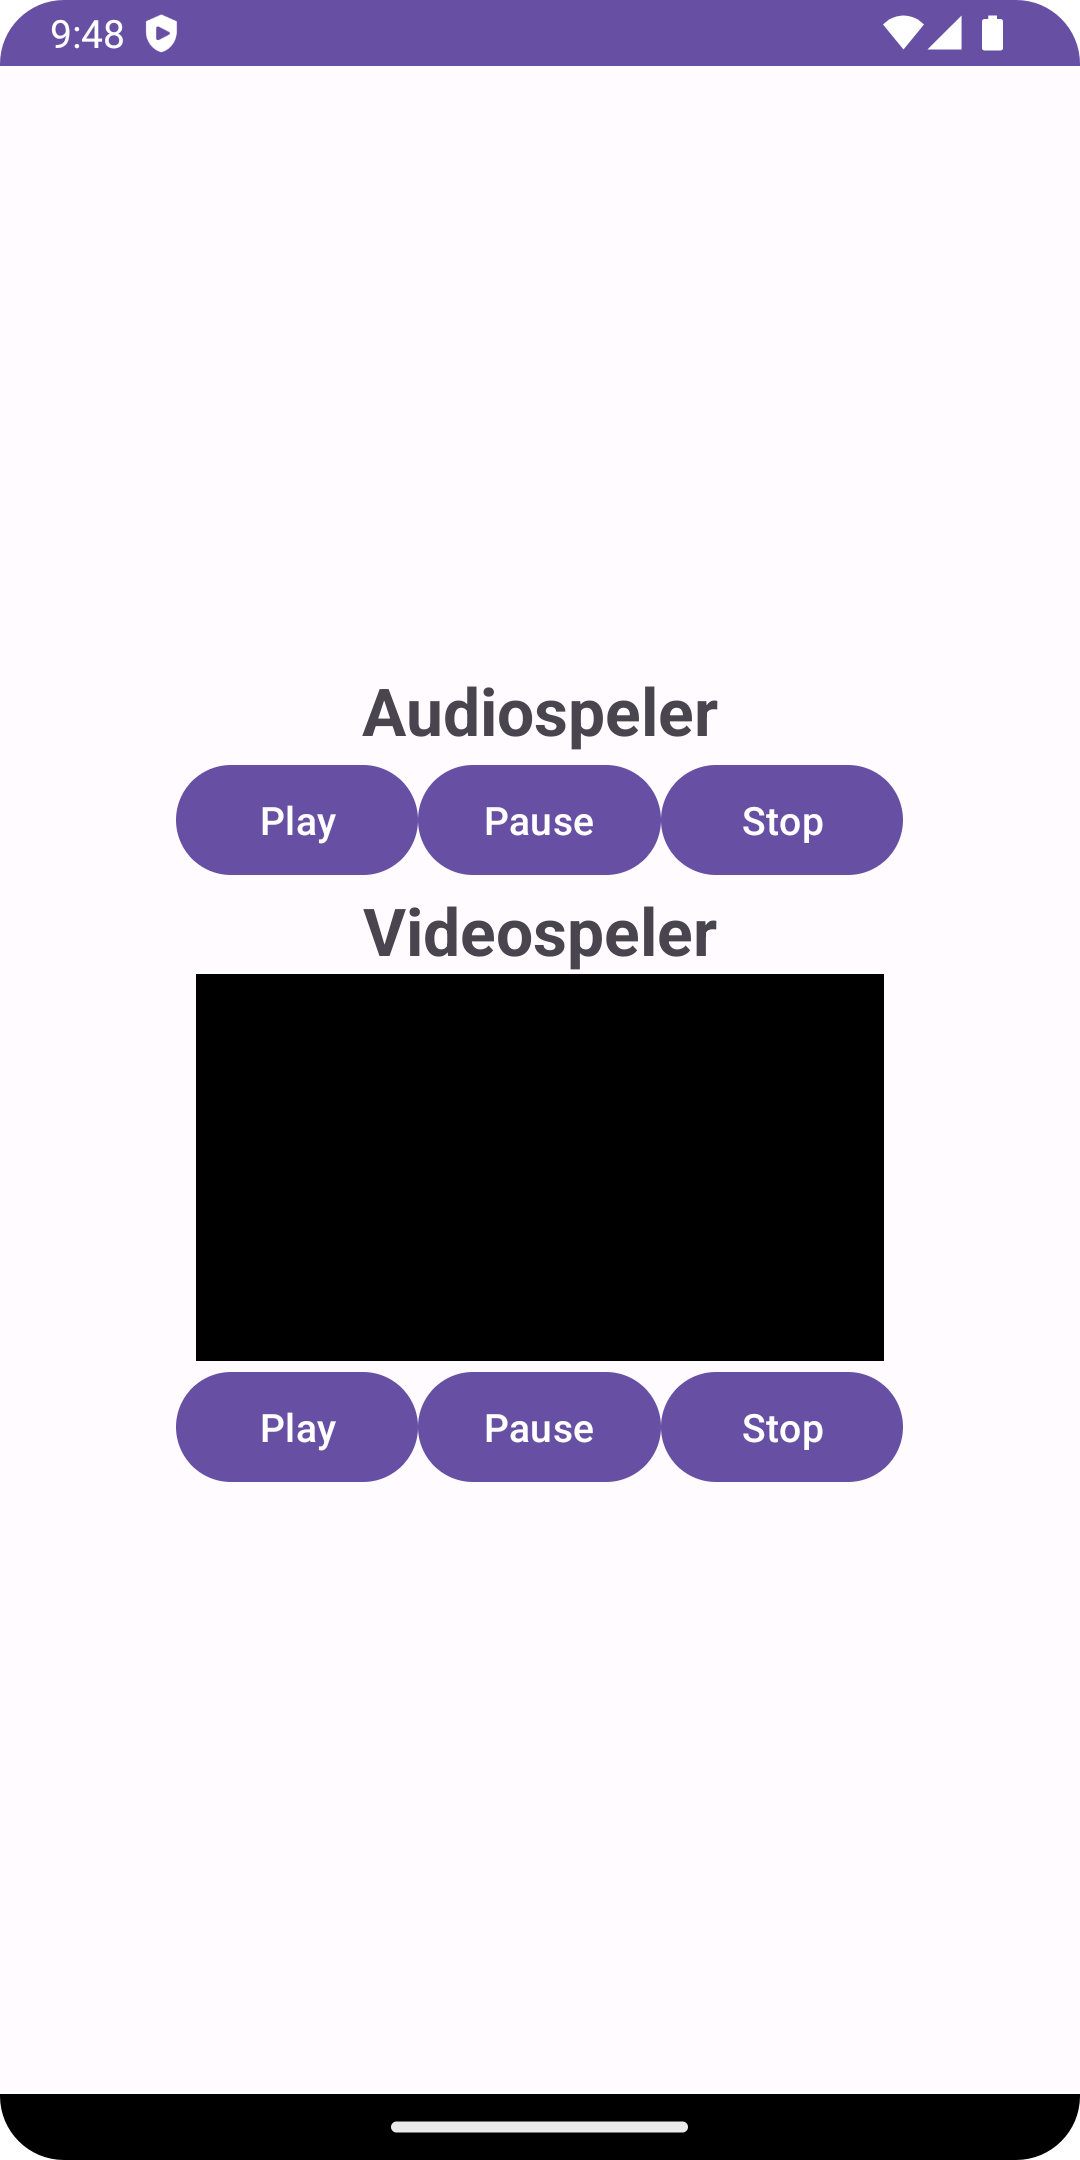
\includegraphics[height=0.4\textheight]{media_layoutnative.png}
    \caption{Layout van applicatie voor het afspelen van audio en video bij Android.}
\end{figure}




